\documentclass{article}

\usepackage{pgf}
%\documentclass{article}

\usepackage{pgf}
\usepackage{tikz}
\usetikzlibrary{arrows, automata}
\usepackage[latin1]{inputenc}
\usepackage{verbatim}

\begin{document}

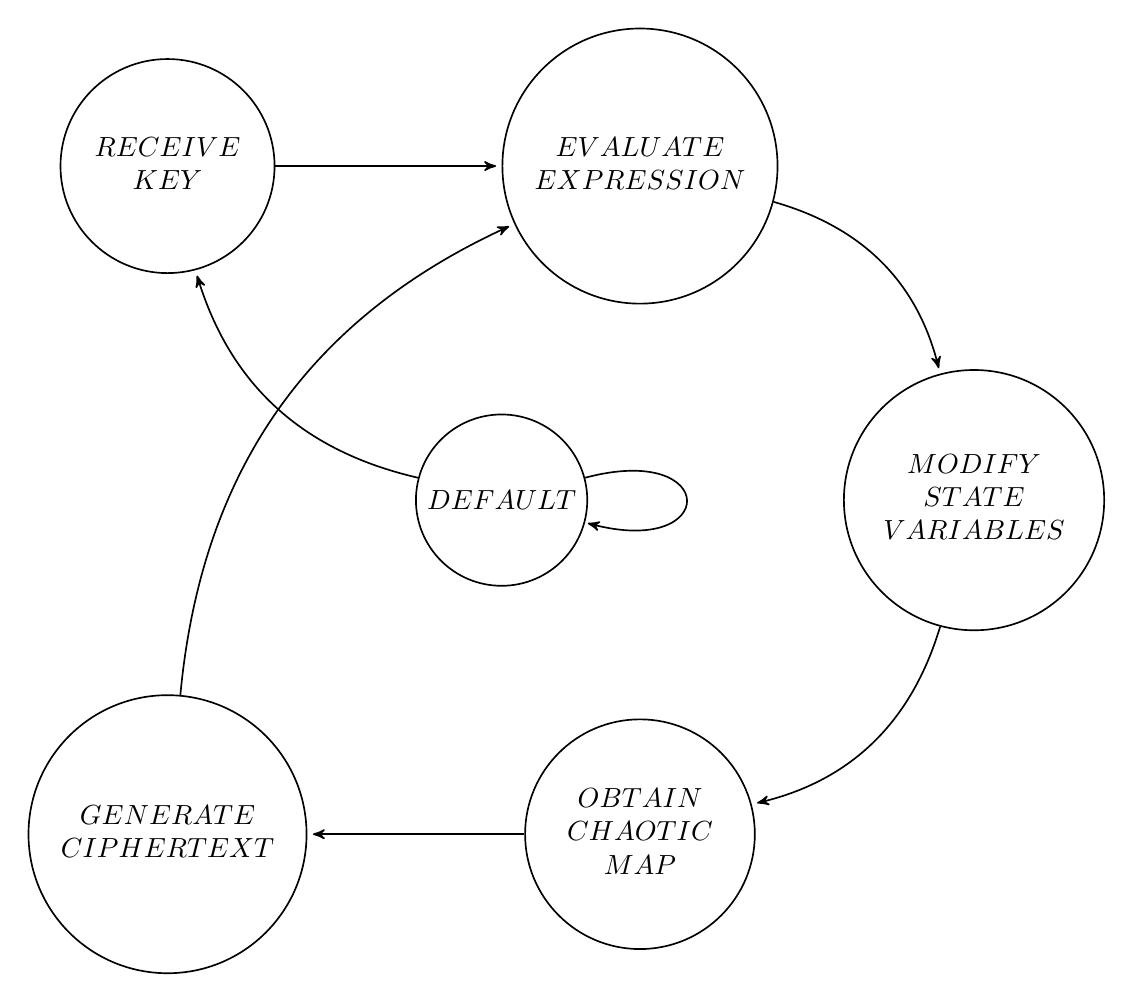
\begin{tikzpicture}[->,>=stealth',shorten >=2pt,auto,node distance=6cm, semithick]
  \tikyle{every state}=[draw=none,text=black]

  \node[state] (A)                         {$DEFAULT$};
  \node[state] (B) [above left of=A]      {\begin{tabular}{c}$RECEIVE$\\$KEY$\end{tabular}};
  \node[state] (C) [right of=B]            {\begin{tabular}{c}$EVALUATE$\\$EXPRESSION$\end{tabular}};
  \node[state] (D) [below right of=C]      {\begin{tabular}{c}$MODIFY$\\$STATE$\\$VARIABLES$\end{tabular}};
  \node[state] (E) [below left of=D]       {\begin{tabular}{c}$OBTAIN$\\$CHAOTIC$\\$MAP$\end{tabular}};
  \node[state] (F) [left of = E]           {\begin{tabular}{c}$GENERATE$\\$CIPHERTEXT$\end{tabular}};
  %\node[state] (G) [left of = F]           {\begin{tabular}{c}$STORE$\\$CIPHERTEXT$\end{tabular}};

\path

(A) edge [loop right] node {} (A)
(B) edge             node {} (C)
(C) edge [bend left] node {} (D)
(D) edge [bend left] node {} (E)
(E) edge             node {} (F)
(F) edge [bend left] node {} (C)
(A) edge [bend left] node {} (B);

\end{tikzpicture}
\end{document}
